\documentclass[a4paper,12pt]{article} 

%%% Работа с русским языком
\usepackage{cmap}					% поиск в PDF
\usepackage{mathtext} 				% русские буквы в фомулах
\usepackage[T2A]{fontenc}			% кодировка
\usepackage[utf8]{inputenc}			% кодировка исходного текста
\usepackage[english,russian]{babel}	% локализация и переносы

%%% Дополнительная работа с математикой
\usepackage{amsmath,amsfonts,amssymb,amsthm,mathtools, gensymb} % AMS
\usepackage{icomma} % "Умная" запятая: $0,2$    ф--- число, $0, 2$ --- перечисление

%%Таблица
\usepackage[table,xcdraw]{xcolor}
\usepackage{caption}
\usepackage{floatrow}
\floatsetup[table]{capposition=top}
\floatsetup[wrapfigure]{capposition=bottom}
\usepackage{multirow}

\usepackage{hyperref}

%Отступы и поля 
\textwidth=18cm
\oddsidemargin=-1cm
\topmargin=-2cm
\textheight=25cm


%% Номера формул
\mathtoolsset{showonlyrefs=false} % Показывать номера только у тех формул, на которые есть \ref{} в тексте.

%% Шрифты
\usepackage{euscript}	 % Шрифт Евклид
\usepackage{mathrsfs} % Красивый матшрифт

%% Свои команды
\DeclareMathOperator{\sgn}{\mathop{sgn}}

%% Перенос знаков в формулах (по Львовскому)
\newcommand*{\hm}[1]{#1\nobreak\discretionary{}
{\hbox{$\mathsurround=0pt #1$}}{}}

%% Стиль страницы
\usepackage{fancyhdr}

%% Для рисунков
\usepackage{graphicx}
\usepackage[export]{adjustbox}
\usepackage{float}
\usepackage{ragged2e}
\usepackage{wrapfig}

\pagestyle{fancy}
\begin{document}
\begin{titlepage}
\begin{center}
%\vspace*{1cm}
\large{\small ФЕДЕРАЛЬНОЕ ГОСУДАРСТВЕННОЕ АВТОНОМНОЕ ОБРАЗОВАТЕЛЬНОЕ\\ УЧРЕЖДЕНИЕ ВЫСШЕГО ОБРАЗОВАНИЯ \\ МОСКОВСКИЙ ФИЗИКО-ТЕХНИЧЕСКИЙ ИНСТИТУТ\\ (НАЦИОНАЛЬНЫЙ ИССЛЕДОВАТЕЛЬСКИЙ УНИВЕРСИТЕТ)\\ ФАКУЛЬТЕТ АЭРОКОСМИЧЕСКИХ ТЕХНОЛОГИЙ}
\vfill
\line(1,0){490}\\[1mm]
\huge{Лабораторная работа 8.1}\\
\huge\textbf{Определение постоянных Стефана–Больцмана и Планка из анализа теплового излучения накаленного тела}\\
\line(1,0){490}\\[1mm]
\vfill
\begin{flushright}
\normalsize{Рогозин Владимир}\\
\normalsize{\textbf{Группа Б03-106}}\\
\end{flushright}
\end{center}
\end{titlepage}
\fancyhead[L] {Работа 8.1}

\textbf{Цель работы}:
При помощи модели абсолютно черного тела (АЧТ) провести измерения температуры оптическим пирометром с исчезающей нитью и термопарой,
исследовать излучение накаленных тел с различной испускательной способностью, определить постоянные Планка и Стефана–Больцмана.


% \textbf{Оборудование}:
% лазер; кассета с набором сеток разного
% периода; линзы; щель с микрометрическим винтом; оптический стол
% c набором рейтеров и крепёжных винтов; экран; линейка.


\section{Теоретические сведения}
Для измерения температуры разогретых тел, удаленных от наблюдателя, применяют методы оптической пирометрии, основанные на использовании зависимости испускательной способности исследуемого тела от температуры. Различают три температуры, функционально связанные с истинной термодинамической температурой и излучательной способностью тела: радиационную $T_\text{рад}$, цветовую $T_\text{цв}$ и яркостную $T_\text{ярк}$.

Под радиационной (энергетической) температурой понимают .

Под цветовой температурой исследуемого тела понимают температуру АЧТ, при которой отношение их спектральных испускательных способностей для двух заданных длин волн одинаково.

Под яркостной температурой понимают температуру АЧТ, при которой его спектральная испускательная способность равна спектральной испускательной способности исследуемого тела при той же длине волны. Именно эту температуру мы будем измерять в данной работе.

Измерение яркостной температуры раскаленного тела производится при помощи оптического пирометра с исчезающей нитью, основанного на визуальном сравнении яркости раскаленной нити с яркостью изображения исследуемого тела. Равенство видимых яркостей, наблюдаемых через монохроматический светофильтр ($\lambda = 650$ нм), фиксируется по исчезновению изображения нити на фоне раскаленного тела. Яркостный метод измерения температуры основан, в соответствии с формулой Планка, на зависимости испускательной способности АЧТ от температуры и длины волны.

Оптический пирометр представляет собой зрительную трубу, внутри которой имеется накаливаемая нить, расположенная в плоскости изображения исследуемого раскаленного тела, а также темно-красный светофильтр ($\lambda = 650$ нм). Через окуляр одновременно наблюдается изображение исследуемого тела и раскаленной нити.

Если в том узком спектральном интервале, который пропускается светофильтром, яркость нити меньше яркости раскаленного тела, то нить видится темной полоской на светлом фоне, и наоборот. При совпадении яркостей нить перестает быть видимой на фоне изображения раскаленного тела. Регулировка яркости нити осуществляется изменением тока, протекающего через нее.

Шкалу прибора, измеряющего ток через нить, предварительно градуируют по АЧТ, термодинамическую температуру которого измеряют с помощью термопары. Если тело излучает не как АЧТ, то определенное значение температуры является яркостной температурой. Яркостная температура тела всегда ниже его термодинамической температуры. Это связано с тем, что любое нечерное тело излучает меньше, чем абсолютно черное тело при той же температуре. Чтобы получить величину термодинамической температуры тела, надо вводить дополнительные поправки, которые определяются для каждого материала экспериментально.

В данной работе используется оптический пирометр с исчезающей нитью, проградуированный при изготовлении по АЧТ, так что его цифровое табло во время измерения высвечивает значение температуры накаленного тела в градусах Цельсия. Вначале с помощью модели АЧТ проверяется правильность работы пирометра, а затем с его помощью исследуется излучение различных материалов и вольфрамовой нити накаливания. Необходимая для обработки проводимых в данной работе измерений зависимость между яркостной и термодинамической температурами вольфрама приведена на рис. \text{\hyperref[fig: T = f(T_br)]{1}}.
\begin{figure}[H]\label{fig: T = f(T_br)}
    \centering
    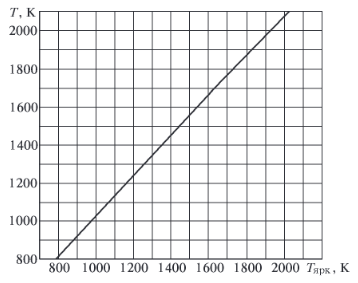
\includegraphics[width = 0.9\textwidth]{T = f(T_br).png}
    \caption{График зависимости $T = f(T_\text{ярк})$ для вольфрама}
\end{figure}

По результатам измерений мощности излучения вольфрамовой нити можно судить о справедливости закона Стефана–Больцмана. Для этого следует мощность, потребляемую нитью, приравнять к излучаемому ею за единицу времени количеству энергии. Если бы нить излучала как АЧТ, то баланс потребляемой и излучаемой энергии определялся бы соотношением
\begin{equation}\label{eq: energy balance BB}
    W = \sigma S(T^4 - T_0^4),
\end{equation}
где W -- потребляемая нитью электрическая мощность, $S$ -- площадь излучающей поверхности нити, $T$ -- температура нити, $T_0$ -- температура окружающей среды. Однако вольфрамовая нить излучает как нечерное тело. Среди нечерных тел выделяются так называемые серые тела, для которых характер распределения излучения совершенно подобен спектру абсолютно черного тела, но излучение ослаблено по сравнению с ним в $\varepsilon_T$ раз для любой длины волны при данной температуре тела $T$.

Если предположить, что нить излучает как серое тело, то выражение (\ref{eq: energy balance BB}) можно записать в виде
\begin{equation}\label{eq: energy balance}
    W = \varepsilon_T\sigma ST^4,
\end{equation}
где уже учтено, что реально температура вольфрама намного выше температуры окружающей среды. Значения коэффициента излучения $\varepsilon_T$ при различных температурах приведены в таблице на рис. \hyperref[fig: Blackness Degree]{2}.

\begin{wrapfigure}[21]{l}{0.45\textwidth}\label{fig: Blackness Degree}
    \begin{center}
    \vspace{-20pt}
        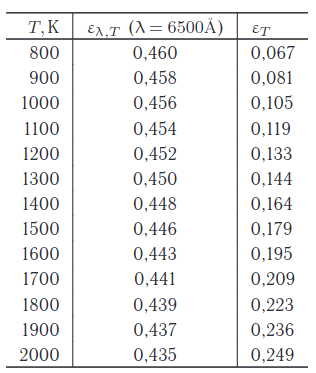
\includegraphics[width = 0.78\textwidth]{Blackness Degree.png}
    \end{center}
    \caption{Поправочные коэффициенты излучения для вольфрама}
\end{wrapfigure}
Измерив температуру вольфрамовой нити в зависимости от подводимой мощности, можно убедиться в справедливости закона Стефана-Больцмана применительно к серому телу.

Из формулы (\ref{eq: energy balance}) можно определить также и величину постоянной $\sigma$ в законе Стефана–Больцмана. Некоторое отличие величин $n$ и $\sigma$, полученных экспериментально, от теоретических значений может быть объяснено особенностью вольфрама, у которого наблюдается селективность излучения в коротковолновом диапазоне. Оказывается, что излучение в видимой области спектра существенно больше, чем это следует из распределения Планка, примененного к серому телу.

Проведя измерения в диапазоне температур от $800$ до $1500$ $\degree$C, можно выяснить, в каком участке этого интервала температур вольфрамовая нить лампы накаливания излучает почти как серое тело, т. е. величины $n$ и $\sigma$ соответствуют теоретическим значениям.

\section{Экспериментальная установка}
Экспериментальная установка (рис. \hyperref[fig: Exp setup]{3}) состоит из оптического пирометра $9$, модели АЧТ, трех исследуемых образцов ($18$, $19$, $20$), блока питания $(1)$ и цифровых вольтметров В7-22А и В7-38.

Пирометр $9$ с исчезающей нитью включает в себя объектив $10$, окуляр $8$, красный светофильтр $4$, позволяющий рассматривать в лучах красного цвета нить пирометра на фоне изображения накаленного исследуемого тела. Перемещение светофильтра осуществляется сектором $12$. Пирометр имеет два диапазона измерений: $700-1200$ $\degree$C и $1200-2000$ $\degree$C. Переключение осуществляется введением серого светофильтра при помощи переключателя $11$ «Включение». регулировка накала нити пирометра выведена на лицевую панель блока питания.

Модель АЧТ представляет собой керамическую трубку диаметром $3$ мм и длиной $50$ мм, закрытую с одного конца и окруженную для теплоизоляции внешним кожухом. Нагрев трубки осуществляется намотанной на ней нихромовой спиралью, питаемой от источника тока. Полость трубки и особенно ее дно излучают практически как абсолютно черное тело. Температура модели АЧТ измеряется хромель-алюмелевой термопарой, один спай которой вмонтирован в дно трубки, а другой находится при комнатной температуре на клемме цифрового вольтметра В7-38, измеряющего ЭДС термопары.

В работе исследуются три образца. Один образец выполнен в виде керамической трубки с набором колец из различных материалов,
нагреваемой изнутри нихромовой спиралью. Материалы колец имеют различную испускательную способность. Спираль подключается к источнику питания $1$ с помощью переключателя $6$ и может нагревать трубку до температуры около $1100$ $\degree$C. Термодинамическая температура колец практически одинакова и равна температуре трубки.

Другой исследуемый образец - вольфрамовая нить электрической лампочки. Она питается от источника $1$, когда переключатель $6$ находится в положении $3$. Сила тока через вольфрамовую нить измеряется с помощью прибора В7-22А ($15$). Падение напряжения на самой нити измеряется непосредственно вольтметром В7-22А ($16$). Таким образом, зная показания обоих приборов, можно определить мощность, потребляемую нитью лампочки.

Источник питания $1$, используемый в работе, снабжен устройством, отключающим в случае перегрузки прибор от потребителя, в этот момент загорается сигнальная лампочка «перегрузка» на передней панели прибора. Если это произойдет, то надо отключить питание прибора от сети $220$ В и уменьшить напряжение на его выходе, а затем повторно включить источник питания.
\begin{figure}[H]\label{fig: Exp setup}
    \centering
    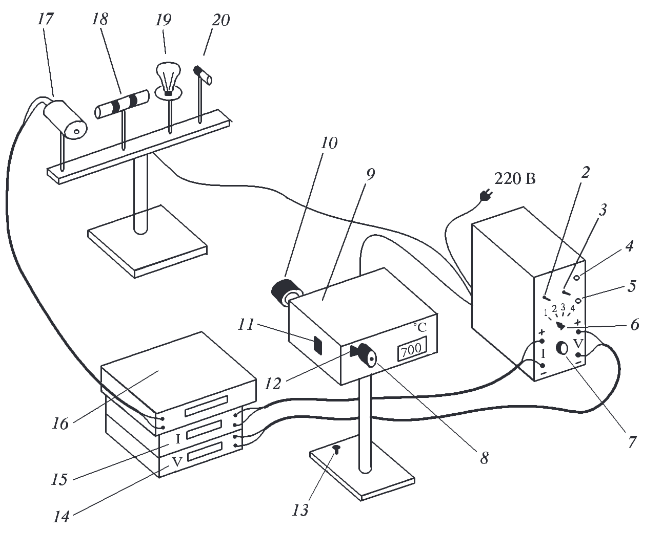
\includegraphics[width = 0.9\textwidth]{Exp setup.png}
    \caption{Схема экспериментальной установки: 1 -- блок питания; 2 -- тумблер включения питания пирометра и образцов; 3 -- тумблер нагрева нити пирометра: «Быстро» -- вверх, «Медленно» -- вниз; 4 -- кнопка «Нагрев нити»; 5 -- кнопка «охлаждение нити»; 6 -- тумблер переключения образцов; 7 -- регулятор мощности нагрева образцов; 8 -- окуляр пирометра; 9 -- корпус пирометра; 10 -- объектив пирометра; 11 -- переключение диапазонов: 700-1200 $\degree$C -- вниз, 1200-2000 $\degree$C -- вверх; 12 -- ручка перемещения красного светофильтра; 13 -- регулировочный винт; 14 -- вольтметр (напряжение на лампе накаливания); 15 -- амперметр (ток через образцы); 16 -- вольтметр в цепи термопары; 17 -- модель АЧТ; 18 -- трубка с кольцами из материалов с разной излучательной способностью; 19 -- лампа накаливания; 20 -- неоновая лампочка}
\end{figure}

\section{Обработка данных}

\subsection{Изучение работы оптического пирометра}
В этой части работы с помощью пирометра измерим температуру модели АЧТ и сравненим её значения со значением температуры, измеренной при помощи термопарного термометра.
\begin{enumerate}
    \item
    Включим питание и нагреем модель АЧТ до температуры $T \sim 1000$ $\degree$C. Также включим цифровой вольметр, чтобы по нему, с помощью термопары, определить температуру АЧТ.
    \item
    Включим питание пирометра и выставим на нём температуру в диапазоне $900-1100$ $\degree$C. Направим пирометр на образец и добьёмся четкого изображения поверхности дна АЧТ. Затем, когда тело достаточно нагрелось, попеременно чередуя увеличение и уменьшение тока накала нити, будем записывать значение температуры, показываемой пирометром при сопадении яркостей АЧТ и вольфрамовой нити. Результаты измерений приведены в таблице ниже.
    \begin{table}[H]\label{tab: BB Temperature}
        \begin{tabular}{|
            >{\columncolor[HTML]{FFFFFF}}c |
            >{\columncolor[HTML]{FFFFFF}}c |
            >{\columncolor[HTML]{FFFFFF}}c |
            >{\columncolor[HTML]{FFFFFF}}c |}
            \hline
            {\color[HTML]{000000} N, номер измерения} & {\color[HTML]{000000} $T$, $\degree$C} & {\color[HTML]{000000} N, номер измерения} & {\color[HTML]{000000} $T$, $\degree$C} \\ \hline
            {\color[HTML]{000000} 1} & {\color[HTML]{000000} 1099} & {\color[HTML]{000000} 4} & {\color[HTML]{000000} 1092} \\ \hline
            {\color[HTML]{000000} 2} & {\color[HTML]{000000} 1091} & {\color[HTML]{000000} 5} & {\color[HTML]{000000} 1097} \\ \hline
            {\color[HTML]{000000} 3} & {\color[HTML]{000000} 1095} & {\color[HTML]{000000} 6} & {\color[HTML]{000000} 1090} \\ \hline
        \end{tabular}
        \caption{Данные измерения яркостной температуры АЧТ}
    \end{table}
    \item 
    Теперь запишем значение напряжение на вольметре, при котором происходили измерения $V = 44,44$ мВ. Сравним температуры АЧТ, измеренные двумя способами: с помощью термопары и с помощью пирометра. Для нахождения первой из  температур воспользуемся формулой перевода напряжения на термопаре в температуру \fbox{$T = V / \alpha$}, где $\alpha = 41$ мкВ/$\degree$C  -- известная постоянная. Таким образом, получаем $T_\text{термоп.} = 1084$ $\degree$C. Заметим, что полученная температура мерилась относительно температуры в комнате $T_0 = 24$ $\degree$C. Значит, истинная температура АЧТ будет равна 
    \[T = T_0 + T_\text{термоп.} = 1108 \text{ } \degree C.\]
    Видим, что полученные различными способами температуры отличаются не более чем на $2\%$, что показывает корректность работы установки.
\end{enumerate}

\subsection{Измерение яркостной температуры накаленных тел}
В этой части работы убедимся, что различные тела, накаленные до одинаковой термодинамической температуры, имеют различную яркостную температуру.
\begin{enumerate}
    \item
    Поставим переключатель 6  в положение 2 «Кольца». После этого дождёмся нагрева керамической трубки с кольцами из различных материалов (до $\approx 900$ $\degree$C).
    \item
    Попробуем измерить яркостную температуру поверхности трубки и каждого из колец. При почти красном калении трубки одно из колец имеет слабо заметное красное свечение, а второе кольцо не светится вообще. Это доказывает, что яркостная температура зависит от материала и в общем случае отличается у двух различных тел, даже при условии, что тела находятся при одинаковой термодинамической температуре. 
\end{enumerate}

\subsection{Проверка закона Стефана–Больцмана}
В этом разделе проверим справедливость закона Стефана–Больцмана. Из экспериментальных данных найдём показатель степени $n$ постоянную Стефана–Больцмана $\sigma$ в законе Стефана-Больцмана, полученные значения сравним с истинными.
\begin{enumerate}
    \item
    Переключим нагрев на лампу накаливания, включим амперметр и вольтметр, с помощью которых будем измерять величину тока и падения напряжения на нити для дальнейшего определения мощности, выделяемой на ней.
    \item
    Теперь будем снимать зависимость силы тока и падения напряжения на нити от её яркостной температуры. Результаты приведены в таблице ниже.
    \begin{table}[H]\label{tab: I and V}
        \begin{tabular}{|
            >{\columncolor[HTML]{FFFFFF}}c |
            >{\columncolor[HTML]{FFFFFF}}c |
            >{\columncolor[HTML]{FFFFFF}}c |}
            \hline
            {\color[HTML]{000000} $T_\text{ярк}$, $\degree$C} & {\color[HTML]{000000} $V$, В} & {\color[HTML]{000000} $I$, А} \\ \hline
            {\color[HTML]{000000} 900}  & {\color[HTML]{000000} 1,92} & {\color[HTML]{000000} 0,503} \\ \hline
            {\color[HTML]{000000} 1000} & {\color[HTML]{000000} 2,62} & {\color[HTML]{000000} 0,579} \\ \hline
            {\color[HTML]{000000} 1100} & {\color[HTML]{000000} 3,84} & {\color[HTML]{000000} 0,698} \\ \hline
            {\color[HTML]{000000} 1200} & {\color[HTML]{000000} 4,55} & {\color[HTML]{000000} 0,761} \\ \hline
            {\color[HTML]{000000} 1300} & {\color[HTML]{000000} 5,93} & {\color[HTML]{000000} 0,874} \\ \hline
            {\color[HTML]{000000} 1400} & {\color[HTML]{000000} 7,12} & {\color[HTML]{000000} 0,963} \\ \hline
            {\color[HTML]{000000} 1500} & {\color[HTML]{000000} 8,34} & {\color[HTML]{000000} 1,047} \\ \hline
            {\color[HTML]{000000} 1600} & {\color[HTML]{000000} 8,98} & {\color[HTML]{000000} 1,091} \\ \hline
        \end{tabular}
        \caption{Падение напряжения и сила тока для различных температур }
    \end{table}
    \item
    С помощью известной зависимости между яркостной и термодинамической температурой вольфрамовой нити $T = g(T_\text{ярк})$ построим зависимость $W = f(T)$. Также, постороив график зависимости $\ln{W} = f_1(\ln{T})$, проверим закон Стефана–Больцмана, используя
    \[\ln{W} = \ln{(\varepsilon_T S \sigma)} + n\ln{T},\]
    определим величину $n$ как тангенс угла наклона прямой в области высоких температур, когда мощность, подводимая к нити, практически полностью расходуется на излучение. Здесь $S = 0,36$ $\text{см}^2$ -- эффективная площадь излучающей поверхности нити лампы при температуре более $1500$ $\degree$C, когда вся нить одинаково накалена. Значение $\varepsilon_T$ для вольфрама берется из \hyperref[fig: Blackness Degree]{таблицы}.
    \item
    Затем найдём величину постоянной Стефана-Больцмана по формуле
    \begin{equation}\label{eq: Stefan-Boltzmann constant}
        \sigma = \frac{W}{\varepsilon_T S T^4}.
    \end{equation}
    Беря в расчёт только точки, для которых температура нити превышала $1700$ K, получим
    \[\fbox{\sigma = (4,58 \pm 0,21)\cdot10^{-8} \text{ } W/ (m^2\cdot K^4), \quad 
    \varepsilon = 4,6\%,}\]
    \[\varepsilon = \frac{4\sigma_T}{T}.\]
    Табличное значение равно $\sigma_\text{табл.} = 5,67\cdot10^{-8} \text{ } W/ (m^2\cdot K^4)$. Отклонение полученного результата от истинного значения составляет $\approx 20\%$.  
    
    \item 
    Теперь вычислим значение постоянной Планка по формуле
    \begin{equation}\label{eq: Plank constant}
        h = \sqrt[3]{\frac{2\pi^5 k_\text{Б}^4}{15c^2\sigma}}.
    \end{equation}
    \[\fbox{h = (7,10 \pm 0,11)\cdot10^{-34} \text{ } J\cdot c, \quad 
    \varepsilon_h = 1,5\%,}\]
    \[\varepsilon = \frac{4\sigma_T}{T}.\]
    Табличное значение равно $h_\text{табл.} = 6,63\cdot10^{-34} \text{ } J\cdot c$. Отклонение полученного результата от истинного значения составляет $\approx 7\%$.  
    
\end{enumerate}

\subsection{Измерение «яркостной температуры» неоновой лампочки}
В данной части работы посмотрим на различие между термодинамической и яркостной температурами неоновой лампочки. 
\begin{enumerate}
    \item
    Подключим неоновую лампочку к сети. После этого, измерим яркостную температуру лампочки: $T_\text{ярк} \approx 750$ $\degree$C. 
    \item 
    Попробуем оценить термодинамическую температуру неоновой лампочки. Дотронувшись до лампочки рукой, убедимся, что термодинамическая температура лампочки не соответствует измеренной яркостной нагретого тела. Это объясняется тем, что неоновая лампа не является АЧТ, а излучает приемущественно на одной частоте  и отражает большую часть падающего на неё излучения.
\end{enumerate}

\section{Вывод}
В данной работе изучалось тепловое излучение нагретых тел. В результате:
\begin{itemize}
    \item
    были измерены яркостные температуры различных тел, которые потом были сравнены с их термодинамическими.  
    \item
    был проверен закон Стефана-Больцмана. Величина показателя степени отличается от истинного значения на $\approx 9\%$, полученное значение постоянной Стефана-Больцмана отличается от табличного на $\approx 20\%$. 
    \item
    из экспериментальных данных была вычислена постоянная Планка. результат совпал с табличным значением с приемлемой точностью $\approx 7\%$. 
    
\end{itemize}

\newpage
%%%%%%%%%%%%%%%%%%%%%%%%% Графики

\begin{figure}[H]\label{fig: W(T)}
    \centering
    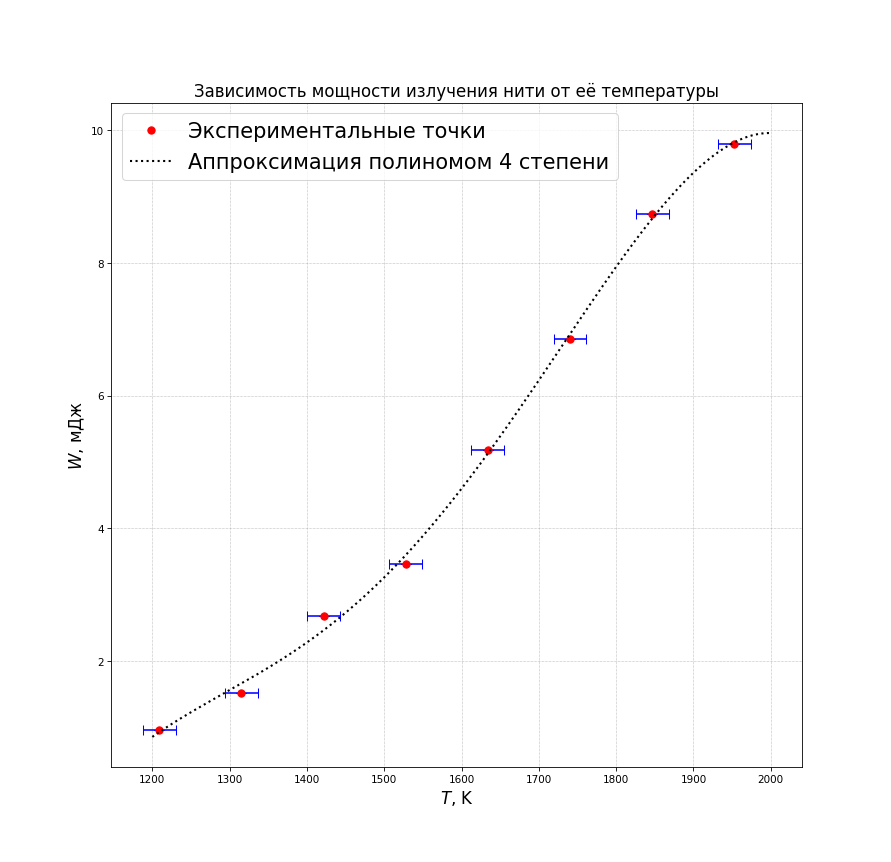
\includegraphics[width = \textwidth]{W(T).png}
\end{figure}
\[y = -6.46\cdot 10^{-14} x^4 + 3,90\cdot 10^{-10} x^3 - 8,66\cdot 10^{-7} x^2 + 8,47\cdot 10^{-4} x  - 3,09\cdot 10^{-1}.\]

\newpage
\begin{figure}[H]\label{fig: lnW(lnT)}
    \centering
    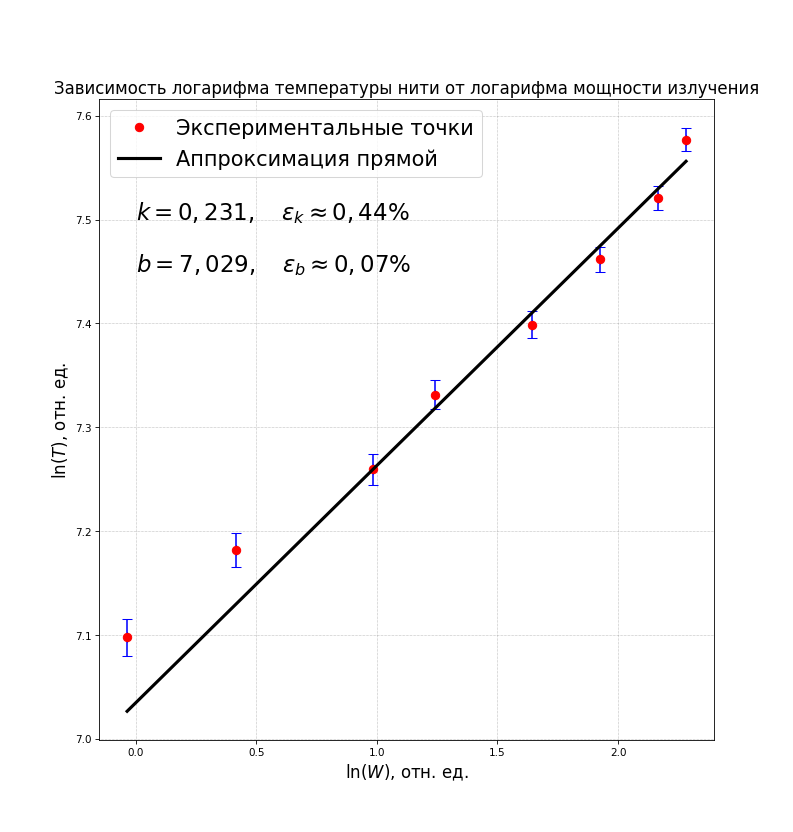
\includegraphics[width = \textwidth]{lnW(lnT).png}
\end{figure}
Аппроксимация была построена методом хи-квадрат без учёта первых двух точек. 
\[n = \frac{1}{k} = (4,33 \pm 0,02), \quad \varepsilon_n = 0,44\% ;\]
\[c = -\frac{b}{k} = -(30,43 \pm 0,13), \quad \varepsilon_c = 0,44\% ;\]
\[\fbox{\ln(W) = n\ln(T) + c}.\]
Коэффициенты прямой и их погрешность были посчитаны методом хи-квадрат для линейной зависимости.

%%%%%%%%%%%%%%%%%%%%%%%%%
\end{document}
